
\documentclass[tikz,border=6pt]{standalone}

\usepackage{amsmath}
\usepackage{tikz}

\usetikzlibrary{calc,angles,quotes}

\begin{document}
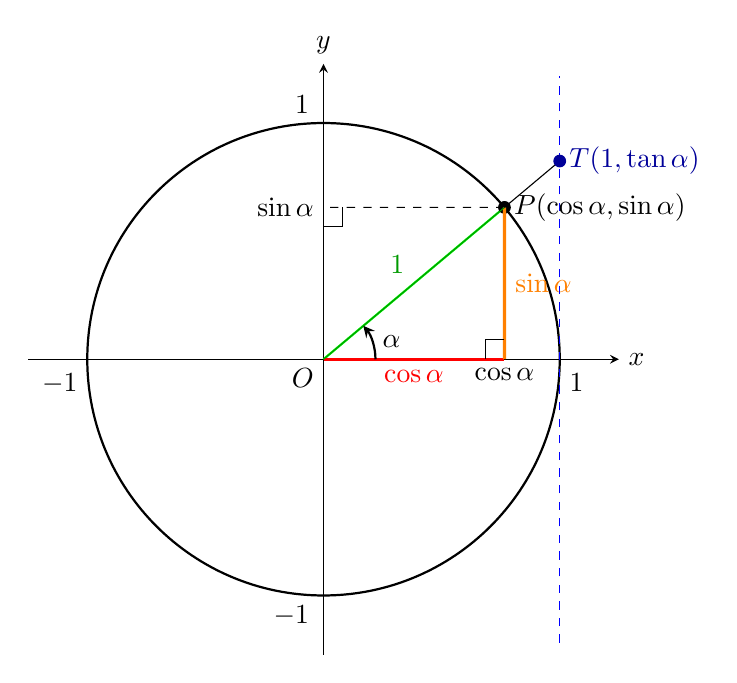
\begin{tikzpicture}[scale=3, >=stealth]

	\def\R{1}
	\def\ang{40} % angle in degrees

	\coordinate (O) at (0,0);
	\coordinate (P) at ({cos(\ang)},{sin(\ang)});
	\coordinate (C) at ({cos(\ang)},0);
	\coordinate (S) at (0,{sin(\ang)});
	\coordinate (T) at (1,{tan(\ang)});

	\node[below left] at ($(O)$) {$O$};

	% axes
	\draw[->] (-1.25,0) -- (1.25,0) node[right] {$x$};
	\draw[->] (0,-1.25) -- (0,1.25) node[above] {$y$};

	% unit circle
	\draw[thick] (O) circle (\R);

	% axis ticks and labels
	\draw (-1,0) -- ++(0,-0.02) node[below left] {$-1$};
	\draw (1,0) -- ++(0,-0.02) node[below right] {$1$};
	\draw (0,-1) -- ++(-0.02,0) node[below left] {$-1$};
	\draw (0,1) -- ++(-0.02,0) node[above left] {$1$};

	% radius to point P
	\draw[thick, green] (O) -- (P);
	\filldraw (P) circle (0.7pt)
	node[right] {$P(\cos\alpha,\sin\alpha)$};

	% projections
	\draw[dashed] (P) -- ({cos(\ang)},0)
	node[below] {$\cos\alpha$};
	\draw[dashed] (P) -- (0,{sin(\ang)})
	node[left] {$\sin\alpha$};

	% colored sine / cosine segments
	\draw[very thick, red]
	(O) -- ({cos(\ang)},0) node[midway, below] {$\cos\alpha$};
	\draw[very thick, orange]
	({cos(\ang)},0) -- (P) node[midway, right] {$\sin\alpha$};

	% angle arc
	\draw[->, thick]
	(0.22,0) arc (0:\ang:0.22)
	node[midway, right] {$\alpha$};

	% tangent line & intersection
	\draw[dashed,blue] (1,-1.2) -- (1,1.2);
	\draw[green!60!black] (O) -- (P)
	node[midway, above left, green!60!black] {$1$};
	\draw[black] (P) -- (T);
	\filldraw[blue!60!black] (T) circle (0.7pt)
	node[right] {$T(1,\tan\alpha)$};

	% right angles
	\pic [draw, angle radius=7pt, angle eccentricity=1]
	{right angle = P--C--O};
	\pic [draw, angle radius=7pt, angle eccentricity=1]
	{right angle = O--S--P};

\end{tikzpicture}
\end{document}
